\begin{frame}
    \frametitle{Python}
    \centering
    
\includegraphics[scale=0.06]{Bin/python_logo.png}

    \vspace{1cm}
    \pause

    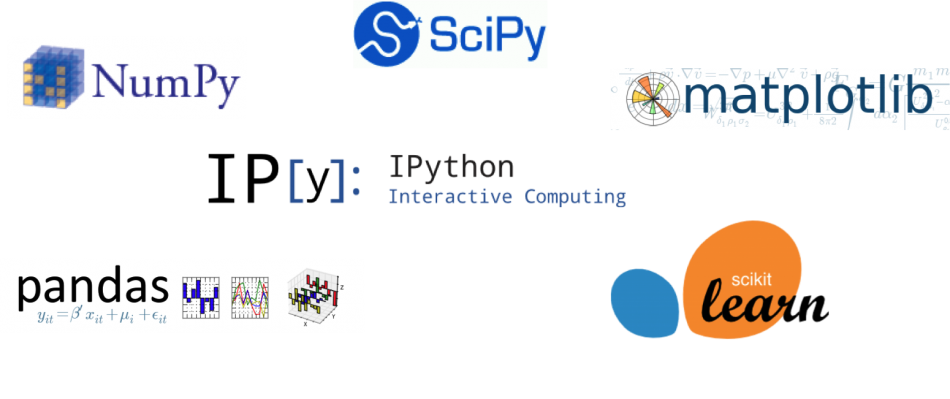
\includegraphics[scale=0.3]{Bin/python_libraries.png}

\end{frame}


\begin{frame}
    \frametitle{Rock-Paper-Scissors}

    \hfuzz = 37pt
    \hspace{3.9cm}
    \vspace{-1cm}
    
\includegraphics[width=.27\textwidth]{Bin/rock-paper-scissors.png}
    \begin{multicols}{3}
        \begin{flushright}
            
\includegraphics[height=0.12\textheight, angle=270]{Bin/rock-paper-scissors.png}
        \end{flushright}
            
        \columnbreak
 
        \begin{equation*}
            \begin{bmatrix}
                0 & & +1 & & -1 \\
                & & & & \\
                -1 & & 0 & & +1 \\
                & & & & \\
                +1 & & -1 & & 0
            \end{bmatrix}
        \end{equation*}

        \columnbreak
        \vfill
    \end{multicols}

\end{frame}



\begin{frame}
    \frametitle{Flit}
    \centering
    \Large 

    \begin{itemize}
        \item Initialising
        \item Packaging
        \item Publishing
    \end{itemize}

\end{frame}



\begin{frame}
    \frametitle{\href{https://pypi.org/}{PyPI} \& \href{https://test.pypi.org/}{TestPyPI}}
    \centering

    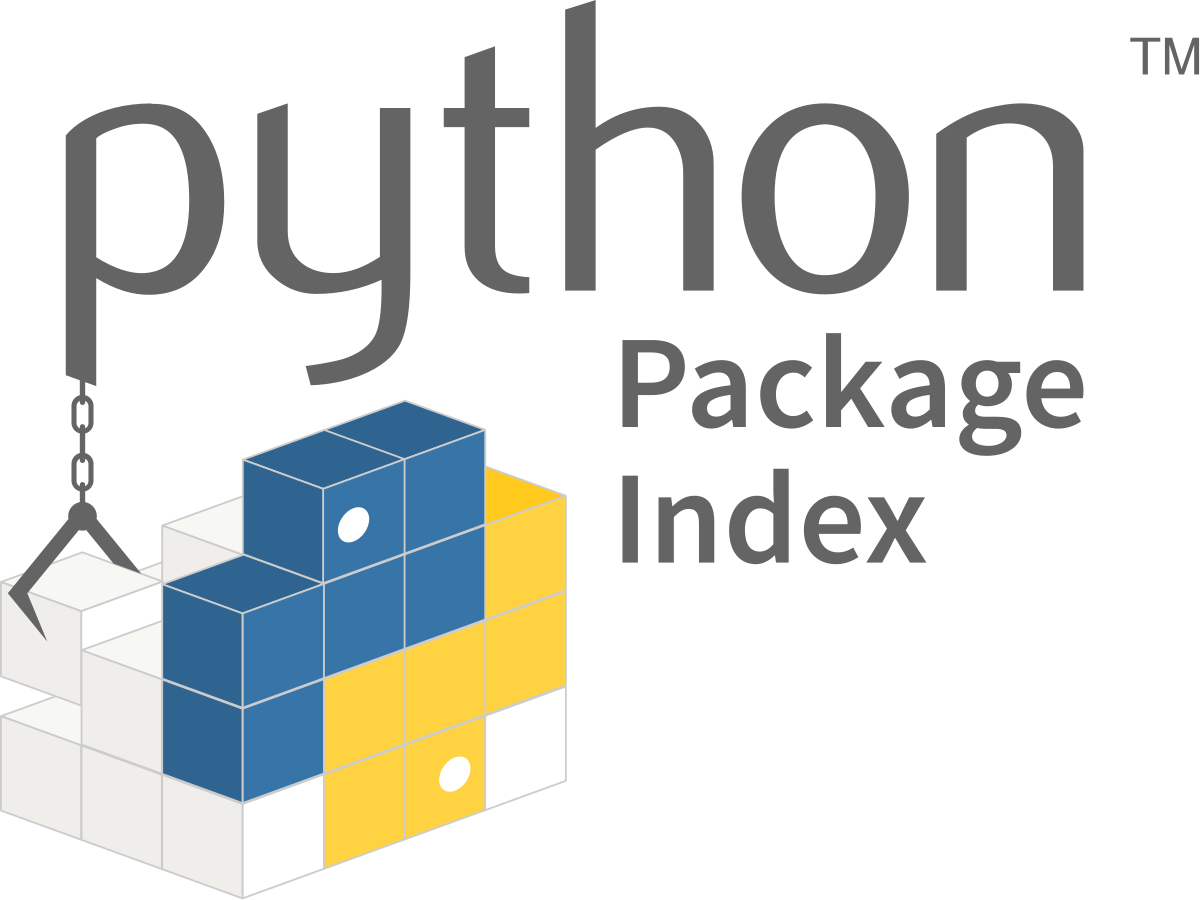
\includegraphics[scale=0.1]{Bin/pypi_logo.png}
\end{frame}
